\documentclass[1p]{elsarticle_modified}
%\bibliographystyle{elsarticle-num}

%\usepackage[colorlinks]{hyperref}
%\usepackage{abbrmath_seonhwa} %\Abb, \Ascr, \Acal ,\Abf, \Afrak
\usepackage{amsfonts}
\usepackage{amssymb}
\usepackage{amsmath}
\usepackage{amsthm}
\usepackage{scalefnt}
\usepackage{amsbsy}
\usepackage{kotex}
\usepackage{caption}
\usepackage{subfig}
\usepackage{color}
\usepackage{graphicx}
\usepackage{xcolor} %% white, black, red, green, blue, cyan, magenta, yellow
\usepackage{float}
\usepackage{setspace}
\usepackage{hyperref}

\usepackage{tikz}
\usetikzlibrary{arrows}

\usepackage{multirow}
\usepackage{array} % fixed length table
\usepackage{hhline}

%%%%%%%%%%%%%%%%%%%%%
\makeatletter
\renewcommand*\env@matrix[1][\arraystretch]{%
	\edef\arraystretch{#1}%
	\hskip -\arraycolsep
	\let\@ifnextchar\new@ifnextchar
	\array{*\c@MaxMatrixCols c}}
\makeatother %https://tex.stackexchange.com/questions/14071/how-can-i-increase-the-line-spacing-in-a-matrix
%%%%%%%%%%%%%%%

\usepackage[normalem]{ulem}

\newcommand{\msout}[1]{\ifmmode\text{\sout{\ensuremath{#1}}}\else\sout{#1}\fi}
%SOURCE: \msout is \stkout macro in https://tex.stackexchange.com/questions/20609/strikeout-in-math-mode

\newcommand{\cancel}[1]{
	\ifmmode
	{\color{red}\msout{#1}}
	\else
	{\color{red}\sout{#1}}
	\fi
}

\newcommand{\add}[1]{
	{\color{blue}\uwave{#1}}
}

\newcommand{\replace}[2]{
	\ifmmode
	{\color{red}\msout{#1}}{\color{blue}\uwave{#2}}
	\else
	{\color{red}\sout{#1}}{\color{blue}\uwave{#2}}
	\fi
}

\newcommand{\Sol}{\mathcal{S}} %segment
\newcommand{\D}{D} %diagram
\newcommand{\A}{\mathcal{A}} %arc


%%%%%%%%%%%%%%%%%%%%%%%%%%%%%5 test

\def\sl{\operatorname{\textup{SL}}(2,\Cbb)}
\def\psl{\operatorname{\textup{PSL}}(2,\Cbb)}
\def\quan{\mkern 1mu \triangleright \mkern 1mu}

\theoremstyle{definition}
\newtheorem{thm}{Theorem}[section]
\newtheorem{prop}[thm]{Proposition}
\newtheorem{lem}[thm]{Lemma}
\newtheorem{ques}[thm]{Question}
\newtheorem{cor}[thm]{Corollary}
\newtheorem{defn}[thm]{Definition}
\newtheorem{exam}[thm]{Example}
\newtheorem{rmk}[thm]{Remark}
\newtheorem{alg}[thm]{Algorithm}

\newcommand{\I}{\sqrt{-1}}
\begin{document}

%\begin{frontmatter}
%
%\title{Boundary parabolic representations of knots up to 8 crossings}
%
%%% Group authors per affiliation:
%\author{Yunhi Cho} 
%\address{Department of Mathematics, University of Seoul, Seoul, Korea}
%\ead{yhcho@uos.ac.kr}
%
%
%\author{Seonhwa Kim} %\fnref{s_kim}}
%\address{Center for Geometry and Physics, Institute for Basic Science, Pohang, 37673, Korea}
%\ead{ryeona17@ibs.re.kr}
%
%\author{Hyuk Kim}
%\address{Department of Mathematical Sciences, Seoul National University, Seoul 08826, Korea}
%\ead{hyukkim@snu.ac.kr}
%
%\author{Seokbeom Yoon}
%\address{Department of Mathematical Sciences, Seoul National University, Seoul, 08826,  Korea}
%\ead{sbyoon15@snu.ac.kr}
%
%\begin{abstract}
%We find all boundary parabolic representation of knots up to 8 crossings.
%
%\end{abstract}
%\begin{keyword}
%    \MSC[2010] 57M25 
%\end{keyword}
%
%\end{frontmatter}

%\linenumbers
%\tableofcontents
%
\newcommand\colored[1]{\textcolor{white}{\rule[-0.35ex]{0.8em}{1.4ex}}\kern-0.8em\color{red} #1}%
%\newcommand\colored[1]{\textcolor{white}{ #1}\kern-2.17ex	\textcolor{white}{ #1}\kern-1.81ex	\textcolor{white}{ #1}\kern-2.15ex\color{red}#1	}

{\Large $\underline{12n_{0257}~(K12n_{0257})}$}

\setlength{\tabcolsep}{10pt}
\renewcommand{\arraystretch}{1.6}
\vspace{1cm}\begin{tabular}{m{100pt}>{\centering\arraybackslash}m{274pt}}
\multirow{5}{120pt}{
	\centering
	\includegraphics[width=112pt]{../../../GIT/diagram.site/Diagrams/png/2346_12n_0257.png}\\
\ \ \ A knot diagram\footnotemark}&
\allowdisplaybreaks
\textbf{Linearized knot diagam} \\
\cline{2-2}
 &
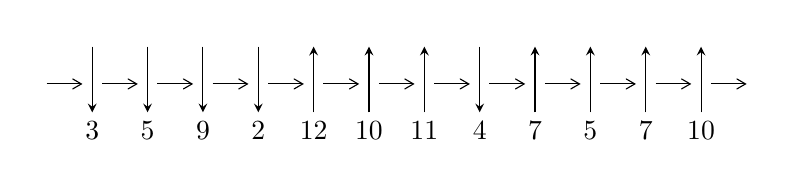
\begin{tikzpicture}[x=20pt, y=17pt]
	% nodes
	\node (C0) at (0, 0) {};
	\node (C1) at (1, 0) {};
	\node (C1U) at (1, +1) {};
	\node (C1D) at (1, -1) {3};

	\node (C2) at (2, 0) {};
	\node (C2U) at (2, +1) {};
	\node (C2D) at (2, -1) {5};

	\node (C3) at (3, 0) {};
	\node (C3U) at (3, +1) {};
	\node (C3D) at (3, -1) {9};

	\node (C4) at (4, 0) {};
	\node (C4U) at (4, +1) {};
	\node (C4D) at (4, -1) {2};

	\node (C5) at (5, 0) {};
	\node (C5U) at (5, +1) {};
	\node (C5D) at (5, -1) {12};

	\node (C6) at (6, 0) {};
	\node (C6U) at (6, +1) {};
	\node (C6D) at (6, -1) {10};

	\node (C7) at (7, 0) {};
	\node (C7U) at (7, +1) {};
	\node (C7D) at (7, -1) {11};

	\node (C8) at (8, 0) {};
	\node (C8U) at (8, +1) {};
	\node (C8D) at (8, -1) {4};

	\node (C9) at (9, 0) {};
	\node (C9U) at (9, +1) {};
	\node (C9D) at (9, -1) {7};

	\node (C10) at (10, 0) {};
	\node (C10U) at (10, +1) {};
	\node (C10D) at (10, -1) {5};

	\node (C11) at (11, 0) {};
	\node (C11U) at (11, +1) {};
	\node (C11D) at (11, -1) {7};

	\node (C12) at (12, 0) {};
	\node (C12U) at (12, +1) {};
	\node (C12D) at (12, -1) {10};
	\node (C13) at (13, 0) {};

	% arrows
	\draw[->,>={angle 60}]
	(C0) edge (C1) (C1) edge (C2) (C2) edge (C3) (C3) edge (C4) (C4) edge (C5) (C5) edge (C6) (C6) edge (C7) (C7) edge (C8) (C8) edge (C9) (C9) edge (C10) (C10) edge (C11) (C11) edge (C12) (C12) edge (C13) ;	\draw[->,>=stealth]
	(C1U) edge (C1D) (C2U) edge (C2D) (C3U) edge (C3D) (C4U) edge (C4D) (C5D) edge (C5U) (C6D) edge (C6U) (C7D) edge (C7U) (C8U) edge (C8D) (C9D) edge (C9U) (C10D) edge (C10U) (C11D) edge (C11U) (C12D) edge (C12U) ;
	\end{tikzpicture} \\
\hhline{~~} \\& 
\textbf{Solving Sequence} \\ \cline{2-2} 
 &
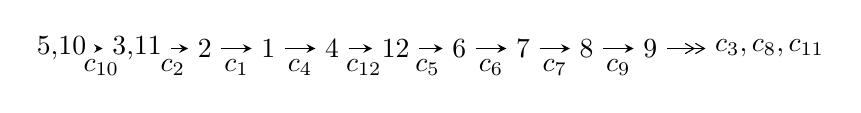
\begin{tikzpicture}[x=23pt, y=7pt]
	% node
	\node (A0) at (-1/8, 0) {5,10};
	\node (A1) at (17/16, 0) {3,11};
	\node (A2) at (17/8, 0) {2};
	\node (A3) at (25/8, 0) {1};
	\node (A4) at (33/8, 0) {4};
	\node (A5) at (41/8, 0) {12};
	\node (A6) at (49/8, 0) {6};
	\node (A7) at (57/8, 0) {7};
	\node (A8) at (65/8, 0) {8};
	\node (A9) at (73/8, 0) {9};
	\node (C1) at (1/2, -1) {$c_{10}$};
	\node (C2) at (13/8, -1) {$c_{2}$};
	\node (C3) at (21/8, -1) {$c_{1}$};
	\node (C4) at (29/8, -1) {$c_{4}$};
	\node (C5) at (37/8, -1) {$c_{12}$};
	\node (C6) at (45/8, -1) {$c_{5}$};
	\node (C7) at (53/8, -1) {$c_{6}$};
	\node (C8) at (61/8, -1) {$c_{7}$};
	\node (C9) at (69/8, -1) {$c_{9}$};
	\node (A10) at (11, 0) {$c_{3},c_{8},c_{11}$};

	% edge
	\draw[->,>=stealth]	
	(A0) edge (A1) (A1) edge (A2) (A2) edge (A3) (A3) edge (A4) (A4) edge (A5) (A5) edge (A6) (A6) edge (A7) (A7) edge (A8) (A8) edge (A9) ;
	\draw[->>,>={angle 60}]	
	(A9) edge (A10);
\end{tikzpicture} \\ 

\end{tabular} \\

\footnotetext{
The image of knot diagram is generated by the software ``\textbf{Draw programme}" developed by Andrew Bartholomew(\url{http://www.layer8.co.uk/maths/draw/index.htm\#Running-draw}), where we modified some parts for our purpose(\url{https://github.com/CATsTAILs/LinksPainter}).
}\phantom \\ \newline 
\centering \textbf{Ideals for irreducible components\footnotemark of $X_{\text{par}}$} 
 
\begin{align*}
I^u_{1}&=\langle 
1.90485\times10^{17} u^{17}-2.51658\times10^{17} u^{16}+\cdots+3.03349\times10^{16} b-4.02818\times10^{17},\\
\phantom{I^u_{1}}&\phantom{= \langle  }2.08713\times10^{17} u^{17}-2.72839\times10^{17} u^{16}+\cdots+7.58374\times10^{15} a-3.96132\times10^{17},\;u^{18}- u^{17}+\cdots-4 u+1\rangle \\
I^u_{2}&=\langle 
3 u^{11}- u^{10}+u^9-9 u^8-6 u^7-3 u^6+4 u^5+18 u^4+12 u^3+7 u^2+b-3 u-3,\\
\phantom{I^u_{2}}&\phantom{= \langle  }-4 u^{11}+3 u^{10}-2 u^9+13 u^8+2 u^7+2 u^6-9 u^5-20 u^4-8 u^3- u^2+a+8 u+4,\\
\phantom{I^u_{2}}&\phantom{= \langle  }u^{12}-3 u^9-3 u^8- u^7+2 u^6+7 u^5+6 u^4+2 u^3-2 u^2-3 u-1\rangle \\
I^u_{3}&=\langle 
u^3+3 u^2+18 b-17 u+46,\;-5 u^3+3 u^2+36 a-41 u-32,\;u^4- u^3+7 u^2+6 u-4\rangle \\
I^u_{4}&=\langle 
2 b+u-1,\;a- u-1,\;u^2+u-1\rangle \\
I^u_{5}&=\langle 
b- u-1,\;-2 u^3+3 u^2+66 a+19 u-1,\;u^4+4 u^3+7 u^2+6 u+11\rangle \\
\\
\end{align*}
\raggedright * 5 irreducible components of $\dim_{\mathbb{C}}=0$, with total 40 representations.\\
\footnotetext{All coefficients of polynomials are rational numbers. But the coefficients are sometimes approximated in decimal forms when there is not enough margin.}
\newpage
\renewcommand{\arraystretch}{1}
\centering \section*{I. $I^u_{1}= \langle 1.90\times10^{17} u^{17}-2.52\times10^{17} u^{16}+\cdots+3.03\times10^{16} b-4.03\times10^{17},\;2.09\times10^{17} u^{17}-2.73\times10^{17} u^{16}+\cdots+7.58\times10^{15} a-3.96\times10^{17},\;u^{18}- u^{17}+\cdots-4 u+1 \rangle$}
\flushleft \textbf{(i) Arc colorings}\\
\begin{tabular}{m{7pt} m{180pt} m{7pt} m{180pt} }
\flushright $a_{5}=$&$\begin{pmatrix}0\\u\end{pmatrix}$ \\
\flushright $a_{10}=$&$\begin{pmatrix}1\\0\end{pmatrix}$ \\
\flushright $a_{3}=$&$\begin{pmatrix}-27.5212 u^{17}+35.9768 u^{16}+\cdots-342.299 u+52.2344\\-6.27938 u^{17}+8.29598 u^{16}+\cdots-84.9277 u+13.2790\end{pmatrix}$ \\
\flushright $a_{11}=$&$\begin{pmatrix}1\\- u^2\end{pmatrix}$ \\
\flushright $a_{2}=$&$\begin{pmatrix}-27.5212 u^{17}+35.9768 u^{16}+\cdots-342.299 u+52.2344\\-11.3536 u^{17}+14.8220 u^{16}+\cdots-146.271 u+21.7346\end{pmatrix}$ \\
\flushright $a_{1}=$&$\begin{pmatrix}-7.55482 u^{17}+8.52485 u^{16}+\cdots-73.2580 u+8.96058\\-1.14106 u^{17}+1.22922 u^{16}+\cdots-9.94123 u+0.881867\end{pmatrix}$ \\
\flushright $a_{4}=$&$\begin{pmatrix}-12.4658 u^{17}+7.03725 u^{16}+\cdots+23.8108 u-25.5769\\-1.03310 u^{17}+1.07235 u^{16}+\cdots-13.6155 u+0.722053\end{pmatrix}$ \\
\flushright $a_{12}=$&$\begin{pmatrix}-6.41376 u^{17}+7.29563 u^{16}+\cdots-63.3168 u+8.07871\\-1.14106 u^{17}+1.22922 u^{16}+\cdots-9.94123 u+0.881867\end{pmatrix}$ \\
\flushright $a_{6}=$&$\begin{pmatrix}6.19684 u^{17}-0.924141 u^{16}+\cdots-69.5089 u+28.5882\\0.881867 u^{17}+0.259189 u^{16}+\cdots-17.5763 u+6.41376\end{pmatrix}$ \\
\flushright $a_{7}=$&$\begin{pmatrix}7.07871 u^{17}-0.664952 u^{16}+\cdots-87.0852 u+35.0020\\0.881867 u^{17}+0.259189 u^{16}+\cdots-17.5763 u+6.41376\end{pmatrix}$ \\
\flushright $a_{8}=$&$\begin{pmatrix}7.07871 u^{17}-0.664952 u^{16}+\cdots-86.0852 u+35.0020\\0.881867 u^{17}+0.259189 u^{16}+\cdots-17.5763 u+6.41376\end{pmatrix}$ \\
\flushright $a_{9}=$&$\begin{pmatrix}22.1744 u^{17}-27.4894 u^{16}+\cdots+263.201 u-35.7652\\5.27270 u^{17}-6.06640 u^{16}+\cdots+53.3756 u-6.19684\end{pmatrix}$\\&\end{tabular}
\flushleft \textbf{(ii) Obstruction class $= -1$}\\~\\
\flushleft \textbf{(iii) Cusp Shapes $= -\frac{2063530662655740221}{30334945780497320} u^{17}+\frac{4790167344610047657}{60669891560994640} u^{16}+\cdots-\frac{39519432929474093823}{60669891560994640} u+\frac{3918064914900190251}{60669891560994640}$}\\~\\
\newpage\renewcommand{\arraystretch}{1}
\flushleft \textbf{(iv) u-Polynomials at the component}\newline \\
\begin{tabular}{m{50pt}|m{274pt}}
Crossings & \hspace{64pt}u-Polynomials at each crossing \\
\hline $$\begin{aligned}c_{1}\end{aligned}$$&$\begin{aligned}
&u^{18}+9 u^{17}+\cdots-656 u+256
\end{aligned}$\\
\hline $$\begin{aligned}c_{2},c_{4}\end{aligned}$$&$\begin{aligned}
&u^{18}-3 u^{17}+\cdots+52 u-16
\end{aligned}$\\
\hline $$\begin{aligned}c_{3},c_{8}\end{aligned}$$&$\begin{aligned}
&u^{18}-5 u^{17}+\cdots+80 u+64
\end{aligned}$\\
\hline $$\begin{aligned}c_{5},c_{6},c_{9}\end{aligned}$$&$\begin{aligned}
&u^{18}+5 u^{16}+\cdots-5 u-1
\end{aligned}$\\
\hline $$\begin{aligned}c_{7},c_{10},c_{11}\end{aligned}$$&$\begin{aligned}
&u^{18}+u^{17}+\cdots+4 u+1
\end{aligned}$\\
\hline $$\begin{aligned}c_{12}\end{aligned}$$&$\begin{aligned}
&u^{18}+12 u^{17}+\cdots+6 u-4
\end{aligned}$\\
\hline
\end{tabular}\\~\\
\newpage\renewcommand{\arraystretch}{1}
\flushleft \textbf{(v) Riley Polynomials at the component}\newline \\
\begin{tabular}{m{50pt}|m{274pt}}
Crossings & \hspace{64pt}Riley Polynomials at each crossing \\
\hline $$\begin{aligned}c_{1}\end{aligned}$$&$\begin{aligned}
&y^{18}+3 y^{17}+\cdots+495872 y+65536
\end{aligned}$\\
\hline $$\begin{aligned}c_{2},c_{4}\end{aligned}$$&$\begin{aligned}
&y^{18}-9 y^{17}+\cdots+656 y+256
\end{aligned}$\\
\hline $$\begin{aligned}c_{3},c_{8}\end{aligned}$$&$\begin{aligned}
&y^{18}+9 y^{17}+\cdots-29440 y+4096
\end{aligned}$\\
\hline $$\begin{aligned}c_{5},c_{6},c_{9}\end{aligned}$$&$\begin{aligned}
&y^{18}+10 y^{17}+\cdots-45 y+1
\end{aligned}$\\
\hline $$\begin{aligned}c_{7},c_{10},c_{11}\end{aligned}$$&$\begin{aligned}
&y^{18}+31 y^{17}+\cdots+6 y+1
\end{aligned}$\\
\hline $$\begin{aligned}c_{12}\end{aligned}$$&$\begin{aligned}
&y^{18}-50 y^{17}+\cdots-2700 y+16
\end{aligned}$\\
\hline
\end{tabular}\\~\\
\newpage\flushleft \textbf{(vi) Complex Volumes and Cusp Shapes}
$$\begin{array}{c|c|c}  
\text{Solutions to }I^u_{1}& \I (\text{vol} + \sqrt{-1}CS) & \text{Cusp shape}\\
 \hline 
\begin{aligned}
u &= -0.584558 + 0.366182 I \\
a &= -0.031695 + 0.764128 I \\
b &= -0.238877 + 0.648680 I\end{aligned}
 & \phantom{-}1.158820 - 0.715487 I & \phantom{-}6.82546 + 3.87567 I \\ \hline\begin{aligned}
u &= -0.584558 - 0.366182 I \\
a &= -0.031695 - 0.764128 I \\
b &= -0.238877 - 0.648680 I\end{aligned}
 & \phantom{-}1.158820 + 0.715487 I & \phantom{-}6.82546 - 3.87567 I \\ \hline\begin{aligned}
u &= \phantom{-}1.51394 + 0.18364 I \\
a &= -0.619867 + 0.808006 I \\
b &= -0.40901 + 1.77160 I\end{aligned}
 & \phantom{-}10.72160 + 4.05902 I & -5.48776 - 6.30227 I \\ \hline\begin{aligned}
u &= \phantom{-}1.51394 - 0.18364 I \\
a &= -0.619867 - 0.808006 I \\
b &= -0.40901 - 1.77160 I\end{aligned}
 & \phantom{-}10.72160 - 4.05902 I & -5.48776 + 6.30227 I \\ \hline\begin{aligned}
u &= -0.022331 + 0.452997 I \\
a &= \phantom{-}1.61941 + 0.40552 I \\
b &= \phantom{-}0.156583 + 0.047051 I\end{aligned}
 & \phantom{-}0.21869 - 2.12649 I & \phantom{-}2.57122 + 5.28808 I \\ \hline\begin{aligned}
u &= -0.022331 - 0.452997 I \\
a &= \phantom{-}1.61941 - 0.40552 I \\
b &= \phantom{-}0.156583 - 0.047051 I\end{aligned}
 & \phantom{-}0.21869 + 2.12649 I & \phantom{-}2.57122 - 5.28808 I \\ \hline\begin{aligned}
u &= \phantom{-}0.025010 + 0.431550 I \\
a &= -1.34703 + 2.60646 I \\
b &= \phantom{-}0.250192 + 0.749320 I\end{aligned}
 & -2.52651 - 6.83690 I & \phantom{-}1.00389 + 11.16505 I \\ \hline\begin{aligned}
u &= \phantom{-}0.025010 - 0.431550 I \\
a &= -1.34703 - 2.60646 I \\
b &= \phantom{-}0.250192 - 0.749320 I\end{aligned}
 & -2.52651 + 6.83690 I & \phantom{-}1.00389 - 11.16505 I \\ \hline\begin{aligned}
u &= \phantom{-}0.007817 + 0.411255 I \\
a &= -0.85304 - 2.78085 I \\
b &= \phantom{-}0.325456 - 0.844226 I\end{aligned}
 & -3.55439 + 1.25550 I & -1.98701 - 1.61045 I \\ \hline\begin{aligned}
u &= \phantom{-}0.007817 - 0.411255 I \\
a &= -0.85304 + 2.78085 I \\
b &= \phantom{-}0.325456 + 0.844226 I\end{aligned}
 & -3.55439 - 1.25550 I & -1.98701 + 1.61045 I\\
 \hline 
 \end{array}$$\newpage$$\begin{array}{c|c|c}  
\text{Solutions to }I^u_{1}& \I (\text{vol} + \sqrt{-1}CS) & \text{Cusp shape}\\
 \hline 
\begin{aligned}
u &= \phantom{-}1.75357\phantom{ +0.000000I} \\
a &= -0.620403\phantom{ +0.000000I} \\
b &= \phantom{-}1.40026\phantom{ +0.000000I}\end{aligned}
 & \phantom{-}7.06782\phantom{ +0.000000I} & -18.1410\phantom{ +0.000000I} \\ \hline\begin{aligned}
u &= \phantom{-}0.204909\phantom{ +0.000000I} \\
a &= \phantom{-}4.38528\phantom{ +0.000000I} \\
b &= \phantom{-}0.536453\phantom{ +0.000000I}\end{aligned}
 & -1.30691\phantom{ +0.000000I} & -9.62130\phantom{ +0.000000I} \\ \hline\begin{aligned}
u &= -1.10465 + 2.31020 I \\
a &= \phantom{-}0.029942 + 0.642788 I \\
b &= \phantom{-}0.31930 + 2.83217 I\end{aligned}
 & -13.4615 - 12.9156 I & \phantom{-0.000000 } 0 \\ \hline\begin{aligned}
u &= -1.10465 - 2.31020 I \\
a &= \phantom{-}0.029942 - 0.642788 I \\
b &= \phantom{-}0.31930 - 2.83217 I\end{aligned}
 & -13.4615 + 12.9156 I & \phantom{-0.000000 } 0 \\ \hline\begin{aligned}
u &= -0.50858 + 2.58223 I \\
a &= \phantom{-}0.535381 - 0.129487 I \\
b &= -0.444741 - 0.317296 I\end{aligned}
 & -8.47225 - 5.66445 I & \phantom{-0.000000 } 0 \\ \hline\begin{aligned}
u &= -0.50858 - 2.58223 I \\
a &= \phantom{-}0.535381 + 0.129487 I \\
b &= -0.444741 + 0.317296 I\end{aligned}
 & -8.47225 + 5.66445 I & \phantom{-0.000000 } 0 \\ \hline\begin{aligned}
u &= \phantom{-}0.19411 + 2.91147 I \\
a &= -0.215532 - 0.577704 I \\
b &= \phantom{-}0.82274 - 2.38447 I\end{aligned}
 & -13.28390 + 2.28868 I & \phantom{-0.000000 } 0 \\ \hline\begin{aligned}
u &= \phantom{-}0.19411 - 2.91147 I \\
a &= -0.215532 + 0.577704 I \\
b &= \phantom{-}0.82274 + 2.38447 I\end{aligned}
 & -13.28390 - 2.28868 I & \phantom{-0.000000 } 0\\
 \hline 
 \end{array}$$\newpage\newpage\renewcommand{\arraystretch}{1}
\centering \section*{II. $I^u_{2}= \langle 3 u^{11}- u^{10}+\cdots+b-3,\;-4 u^{11}+3 u^{10}+\cdots+a+4,\;u^{12}-3 u^9+\cdots-3 u-1 \rangle$}
\flushleft \textbf{(i) Arc colorings}\\
\begin{tabular}{m{7pt} m{180pt} m{7pt} m{180pt} }
\flushright $a_{5}=$&$\begin{pmatrix}0\\u\end{pmatrix}$ \\
\flushright $a_{10}=$&$\begin{pmatrix}1\\0\end{pmatrix}$ \\
\flushright $a_{3}=$&$\begin{pmatrix}4 u^{11}-3 u^{10}+\cdots-8 u-4\\-3 u^{11}+u^{10}+\cdots+3 u+3\end{pmatrix}$ \\
\flushright $a_{11}=$&$\begin{pmatrix}1\\- u^2\end{pmatrix}$ \\
\flushright $a_{2}=$&$\begin{pmatrix}4 u^{11}-3 u^{10}+\cdots-8 u-4\\-5 u^{11}+2 u^{10}+\cdots+8 u+6\end{pmatrix}$ \\
\flushright $a_{1}=$&$\begin{pmatrix}-3 u^{11}+u^{10}+9 u^8+6 u^7-7 u^5-19 u^4-11 u^3- u^2+8 u+6\\- u^2-1\end{pmatrix}$ \\
\flushright $a_{4}=$&$\begin{pmatrix}-6 u^{11}+4 u^{10}+\cdots+14 u+8\\7 u^{11}-5 u^{10}+\cdots-21 u-13\end{pmatrix}$ \\
\flushright $a_{12}=$&$\begin{pmatrix}-3 u^{11}+u^{10}+9 u^8+6 u^7-7 u^5-19 u^4-11 u^3+8 u+7\\- u^2-1\end{pmatrix}$ \\
\flushright $a_{6}=$&$\begin{pmatrix}7 u^{11}-3 u^{10}+\cdots-14 u-13\\- u^{11}+3 u^8+3 u^7+u^6-2 u^5-7 u^4-6 u^3-2 u^2+2 u+3\end{pmatrix}$ \\
\flushright $a_{7}=$&$\begin{pmatrix}6 u^{11}-3 u^{10}+u^9-18 u^8-9 u^7+12 u^5+35 u^4+17 u^3+u^2-12 u-10\\- u^{11}+3 u^8+3 u^7+u^6-2 u^5-7 u^4-6 u^3-2 u^2+2 u+3\end{pmatrix}$ \\
\flushright $a_{8}=$&$\begin{pmatrix}6 u^{11}-3 u^{10}+u^9-18 u^8-9 u^7+12 u^5+35 u^4+17 u^3+u^2-13 u-10\\- u^{11}+3 u^8+3 u^7+u^6-2 u^5-7 u^4-5 u^3-2 u^2+2 u+3\end{pmatrix}$ \\
\flushright $a_{9}=$&$\begin{pmatrix}10 u^{11}-6 u^{10}+\cdots-21 u-17\\-3 u^{11}+u^{10}+9 u^8+6 u^7-7 u^5-19 u^4-11 u^3+8 u+7\end{pmatrix}$\\&\end{tabular}
\flushleft \textbf{(ii) Obstruction class $= 1$}\\~\\
\flushleft \textbf{(iii) Cusp Shapes $= 12 u^{11}-12 u^{10}+3 u^9-41 u^8+15 u^6+38 u^5+73 u^4- u^3-22 u^2-57 u-30$}\\~\\
\newpage\renewcommand{\arraystretch}{1}
\flushleft \textbf{(iv) u-Polynomials at the component}\newline \\
\begin{tabular}{m{50pt}|m{274pt}}
Crossings & \hspace{64pt}u-Polynomials at each crossing \\
\hline $$\begin{aligned}c_{1}\end{aligned}$$&$\begin{aligned}
&u^{12}-4 u^{11}+\cdots-13 u+1
\end{aligned}$\\
\hline $$\begin{aligned}c_{2}\end{aligned}$$&$\begin{aligned}
&u^{12}+4 u^{11}+\cdots- u+1
\end{aligned}$\\
\hline $$\begin{aligned}c_{3}\end{aligned}$$&$\begin{aligned}
&u^{12}+6 u^{10}+3 u^9+13 u^8+7 u^7+15 u^6+6 u^5+2 u^3-2 u^2-3 u+1
\end{aligned}$\\
\hline $$\begin{aligned}c_{4}\end{aligned}$$&$\begin{aligned}
&u^{12}-4 u^{11}+\cdots+u+1
\end{aligned}$\\
\hline $$\begin{aligned}c_{5},c_{9}\end{aligned}$$&$\begin{aligned}
&u^{12}-3 u^{11}+2 u^{10}+2 u^9-6 u^8+7 u^7-2 u^6- u^5+3 u^4-3 u^3-1
\end{aligned}$\\
\hline $$\begin{aligned}c_{6}\end{aligned}$$&$\begin{aligned}
&u^{12}+3 u^{11}+2 u^{10}-2 u^9-6 u^8-7 u^7-2 u^6+u^5+3 u^4+3 u^3-1
\end{aligned}$\\
\hline $$\begin{aligned}c_{7},c_{10}\end{aligned}$$&$\begin{aligned}
&u^{12}-3 u^9-3 u^8- u^7+2 u^6+7 u^5+6 u^4+2 u^3-2 u^2-3 u-1
\end{aligned}$\\
\hline $$\begin{aligned}c_{8}\end{aligned}$$&$\begin{aligned}
&u^{12}+6 u^{10}-3 u^9+13 u^8-7 u^7+15 u^6-6 u^5-2 u^3-2 u^2+3 u+1
\end{aligned}$\\
\hline $$\begin{aligned}c_{11}\end{aligned}$$&$\begin{aligned}
&u^{12}+3 u^9-3 u^8+u^7+2 u^6-7 u^5+6 u^4-2 u^3-2 u^2+3 u-1
\end{aligned}$\\
\hline $$\begin{aligned}c_{12}\end{aligned}$$&$\begin{aligned}
&u^{12}-12 u^{11}+\cdots-12 u+9
\end{aligned}$\\
\hline
\end{tabular}\\~\\
\newpage\renewcommand{\arraystretch}{1}
\flushleft \textbf{(v) Riley Polynomials at the component}\newline \\
\begin{tabular}{m{50pt}|m{274pt}}
Crossings & \hspace{64pt}Riley Polynomials at each crossing \\
\hline $$\begin{aligned}c_{1}\end{aligned}$$&$\begin{aligned}
&y^{12}+12 y^{11}+\cdots-81 y+1
\end{aligned}$\\
\hline $$\begin{aligned}c_{2},c_{4}\end{aligned}$$&$\begin{aligned}
&y^{12}-4 y^{11}+\cdots-13 y+1
\end{aligned}$\\
\hline $$\begin{aligned}c_{3},c_{8}\end{aligned}$$&$\begin{aligned}
&y^{12}+12 y^{11}+\cdots-13 y+1
\end{aligned}$\\
\hline $$\begin{aligned}c_{5},c_{6},c_{9}\end{aligned}$$&$\begin{aligned}
&y^{12}-5 y^{11}+4 y^{10}+10 y^9-27 y^7-8 y^6+25 y^5+15 y^4-5 y^3-6 y^2+1
\end{aligned}$\\
\hline $$\begin{aligned}c_{7},c_{10},c_{11}\end{aligned}$$&$\begin{aligned}
&y^{12}-6 y^{10}-5 y^9+15 y^8+25 y^7-8 y^6-27 y^5+10 y^3+4 y^2-5 y+1
\end{aligned}$\\
\hline $$\begin{aligned}c_{12}\end{aligned}$$&$\begin{aligned}
&y^{12}-24 y^{11}+\cdots-234 y+81
\end{aligned}$\\
\hline
\end{tabular}\\~\\
\newpage\flushleft \textbf{(vi) Complex Volumes and Cusp Shapes}
$$\begin{array}{c|c|c}  
\text{Solutions to }I^u_{2}& \I (\text{vol} + \sqrt{-1}CS) & \text{Cusp shape}\\
 \hline 
\begin{aligned}
u &= -0.366604 + 0.825368 I \\
a &= \phantom{-}1.11814 + 0.91713 I \\
b &= -0.413716 + 0.377477 I\end{aligned}
 & -2.86185 + 6.14960 I & -3.55511 - 1.94828 I \\ \hline\begin{aligned}
u &= -0.366604 - 0.825368 I \\
a &= \phantom{-}1.11814 - 0.91713 I \\
b &= -0.413716 - 0.377477 I\end{aligned}
 & -2.86185 - 6.14960 I & -3.55511 + 1.94828 I \\ \hline\begin{aligned}
u &= -0.851892\phantom{ +0.000000I} \\
a &= -0.391239\phantom{ +0.000000I} \\
b &= -2.26079\phantom{ +0.000000I}\end{aligned}
 & \phantom{-}3.56755\phantom{ +0.000000I} & \phantom{-}13.7860\phantom{ +0.000000I} \\ \hline\begin{aligned}
u &= \phantom{-}0.111536 + 1.194340 I \\
a &= \phantom{-}0.317924 - 0.704003 I \\
b &= -0.993719 + 0.895794 I\end{aligned}
 & -5.28057 - 0.69048 I & -8.92309 + 4.67234 I \\ \hline\begin{aligned}
u &= \phantom{-}0.111536 - 1.194340 I \\
a &= \phantom{-}0.317924 + 0.704003 I \\
b &= -0.993719 - 0.895794 I\end{aligned}
 & -5.28057 + 0.69048 I & -8.92309 - 4.67234 I \\ \hline\begin{aligned}
u &= \phantom{-}0.765921\phantom{ +0.000000I} \\
a &= \phantom{-}1.24205\phantom{ +0.000000I} \\
b &= -9.03089\phantom{ +0.000000I}\end{aligned}
 & \phantom{-}2.40622\phantom{ +0.000000I} & -53.6250\phantom{ +0.000000I} \\ \hline\begin{aligned}
u &= -0.496770 + 1.152800 I \\
a &= -0.554307 + 0.648652 I \\
b &= \phantom{-}0.388509 + 0.841432 I\end{aligned}
 & -0.483582 + 0.496104 I & -0.592681 - 0.118839 I \\ \hline\begin{aligned}
u &= -0.496770 - 1.152800 I \\
a &= -0.554307 - 0.648652 I \\
b &= \phantom{-}0.388509 - 0.841432 I\end{aligned}
 & -0.483582 - 0.496104 I & -0.592681 + 0.118839 I \\ \hline\begin{aligned}
u &= -0.629825 + 0.069225 I \\
a &= \phantom{-}1.33711 - 0.51168 I \\
b &= -0.874744 + 0.682079 I\end{aligned}
 & \phantom{-}4.44304 + 1.79476 I & \phantom{-}4.83493 - 4.62713 I \\ \hline\begin{aligned}
u &= -0.629825 - 0.069225 I \\
a &= \phantom{-}1.33711 + 0.51168 I \\
b &= -0.874744 - 0.682079 I\end{aligned}
 & \phantom{-}4.44304 - 1.79476 I & \phantom{-}4.83493 + 4.62713 I\\
 \hline 
 \end{array}$$\newpage$$\begin{array}{c|c|c}  
\text{Solutions to }I^u_{2}& \I (\text{vol} + \sqrt{-1}CS) & \text{Cusp shape}\\
 \hline 
\begin{aligned}
u &= \phantom{-}1.42465 + 0.18625 I \\
a &= -0.644266 + 0.830701 I \\
b &= -0.46049 + 1.87154 I\end{aligned}
 & \phantom{-}11.06570 + 3.92660 I & \phantom{-}15.1553 + 1.2084 I \\ \hline\begin{aligned}
u &= \phantom{-}1.42465 - 0.18625 I \\
a &= -0.644266 - 0.830701 I \\
b &= -0.46049 - 1.87154 I\end{aligned}
 & \phantom{-}11.06570 - 3.92660 I & \phantom{-}15.1553 - 1.2084 I\\
 \hline 
 \end{array}$$\newpage\newpage\renewcommand{\arraystretch}{1}
\centering \section*{III. $I^u_{3}= \langle u^3+3 u^2+18 b-17 u+46,\;-5 u^3+3 u^2+36 a-41 u-32,\;u^4- u^3+7 u^2+6 u-4 \rangle$}
\flushleft \textbf{(i) Arc colorings}\\
\begin{tabular}{m{7pt} m{180pt} m{7pt} m{180pt} }
\flushright $a_{5}=$&$\begin{pmatrix}0\\u\end{pmatrix}$ \\
\flushright $a_{10}=$&$\begin{pmatrix}1\\0\end{pmatrix}$ \\
\flushright $a_{3}=$&$\begin{pmatrix}\frac{5}{36} u^3-\frac{1}{12} u^2+\frac{41}{36} u+\frac{8}{9}\\-\frac{1}{18} u^3-\frac{1}{6} u^2+\frac{17}{18} u-\frac{23}{9}\end{pmatrix}$ \\
\flushright $a_{11}=$&$\begin{pmatrix}1\\- u^2\end{pmatrix}$ \\
\flushright $a_{2}=$&$\begin{pmatrix}\frac{5}{36} u^3-\frac{1}{12} u^2+\frac{41}{36} u+\frac{8}{9}\\-\frac{5}{18} u^3+\frac{1}{6} u^2+\frac{13}{18} u-\frac{25}{9}\end{pmatrix}$ \\
\flushright $a_{1}=$&$\begin{pmatrix}\frac{1}{9} u^3-\frac{1}{6} u^2+\frac{11}{18} u+\frac{11}{18}\\-\frac{1}{18} u^3-\frac{1}{6} u^2-\frac{1}{18} u-\frac{14}{9}\end{pmatrix}$ \\
\flushright $a_{4}=$&$\begin{pmatrix}\frac{1}{9} u^3-\frac{1}{6} u^2+\frac{11}{18} u+\frac{11}{18}\\\frac{7}{18} u^3-\frac{5}{6} u^2+\frac{7}{18} u-\frac{10}{9}\end{pmatrix}$ \\
\flushright $a_{12}=$&$\begin{pmatrix}\frac{1}{6} u^3+\frac{2}{3} u+\frac{13}{6}\\-\frac{1}{18} u^3-\frac{1}{6} u^2-\frac{1}{18} u-\frac{14}{9}\end{pmatrix}$ \\
\flushright $a_{6}=$&$\begin{pmatrix}\frac{5}{12} u^3-\frac{1}{4} u^2+\frac{29}{12} u+\frac{5}{3}\\-\frac{5}{18} u^3+\frac{1}{6} u^2-\frac{23}{18} u-\frac{7}{9}\end{pmatrix}$ \\
\flushright $a_{7}=$&$\begin{pmatrix}\frac{5}{36} u^3-\frac{1}{12} u^2+\frac{41}{36} u+\frac{8}{9}\\-\frac{5}{18} u^3+\frac{1}{6} u^2-\frac{23}{18} u-\frac{7}{9}\end{pmatrix}$ \\
\flushright $a_{8}=$&$\begin{pmatrix}\frac{1}{12} u^3-\frac{1}{4} u^2+\frac{1}{12} u+\frac{1}{3}\\\frac{11}{18} u^3-\frac{7}{6} u^2-\frac{43}{18} u+\frac{1}{9}\end{pmatrix}$ \\
\flushright $a_{9}=$&$\begin{pmatrix}-\frac{1}{9} u^3+\frac{1}{6} u^2-\frac{11}{18} u-\frac{11}{18}\\-\frac{1}{6} u^3+\frac{1}{2} u^2+\frac{5}{6} u+\frac{4}{3}\end{pmatrix}$\\&\end{tabular}
\flushleft \textbf{(ii) Obstruction class $= -1$}\\~\\
\flushleft \textbf{(iii) Cusp Shapes $= -2$}\\~\\
\newpage\renewcommand{\arraystretch}{1}
\flushleft \textbf{(iv) u-Polynomials at the component}\newline \\
\begin{tabular}{m{50pt}|m{274pt}}
Crossings & \hspace{64pt}u-Polynomials at each crossing \\
\hline $$\begin{aligned}c_{1}\end{aligned}$$&$\begin{aligned}
&(u^2+3 u+1)^2
\end{aligned}$\\
\hline $$\begin{aligned}c_{2},c_{4},c_{12}\end{aligned}$$&$\begin{aligned}
&(u^2- u-1)^2
\end{aligned}$\\
\hline $$\begin{aligned}c_{3},c_{8}\end{aligned}$$&$\begin{aligned}
&(u^2+u-1)^2
\end{aligned}$\\
\hline $$\begin{aligned}c_{5},c_{6},c_{9}\end{aligned}$$&$\begin{aligned}
&u^4+4 u^3+5 u^2-8 u-11
\end{aligned}$\\
\hline $$\begin{aligned}c_{7},c_{10},c_{11}\end{aligned}$$&$\begin{aligned}
&u^4+u^3+7 u^2-6 u-4
\end{aligned}$\\
\hline
\end{tabular}\\~\\
\newpage\renewcommand{\arraystretch}{1}
\flushleft \textbf{(v) Riley Polynomials at the component}\newline \\
\begin{tabular}{m{50pt}|m{274pt}}
Crossings & \hspace{64pt}Riley Polynomials at each crossing \\
\hline $$\begin{aligned}c_{1}\end{aligned}$$&$\begin{aligned}
&(y^2-7 y+1)^2
\end{aligned}$\\
\hline $$\begin{aligned}c_{2},c_{3},c_{4}\\c_{8},c_{12}\end{aligned}$$&$\begin{aligned}
&(y^2-3 y+1)^2
\end{aligned}$\\
\hline $$\begin{aligned}c_{5},c_{6},c_{9}\end{aligned}$$&$\begin{aligned}
&y^4-6 y^3+67 y^2-174 y+121
\end{aligned}$\\
\hline $$\begin{aligned}c_{7},c_{10},c_{11}\end{aligned}$$&$\begin{aligned}
&y^4+13 y^3+53 y^2-92 y+16
\end{aligned}$\\
\hline
\end{tabular}\\~\\
\newpage\flushleft \textbf{(vi) Complex Volumes and Cusp Shapes}
$$\begin{array}{c|c|c}  
\text{Solutions to }I^u_{3}& \I (\text{vol} + \sqrt{-1}CS) & \text{Cusp shape}\\
 \hline 
\begin{aligned}
u &= -1.06243\phantom{ +0.000000I} \\
a &= -0.581719\phantom{ +0.000000I} \\
b &= -3.68046\phantom{ +0.000000I}\end{aligned}
 & \phantom{-}2.96088\phantom{ +0.000000I} & -2.00000\phantom{ +0.000000I} \\ \hline\begin{aligned}
u &= \phantom{-}0.444394\phantom{ +0.000000I} \\
a &= \phantom{-}1.39074\phantom{ +0.000000I} \\
b &= -2.17364\phantom{ +0.000000I}\end{aligned}
 & \phantom{-}2.96088\phantom{ +0.000000I} & -2.00000\phantom{ +0.000000I} \\ \hline\begin{aligned}
u &= \phantom{-}0.80902 + 2.79600 I \\
a &= -0.154508 + 0.533989 I \\
b &= \phantom{-}0.42705 + 2.79600 I\end{aligned}
 & -12.8305\phantom{ +0.000000I} & -2.00000\phantom{ +0.000000I} \\ \hline\begin{aligned}
u &= \phantom{-}0.80902 - 2.79600 I \\
a &= -0.154508 - 0.533989 I \\
b &= \phantom{-}0.42705 - 2.79600 I\end{aligned}
 & -12.8305\phantom{ +0.000000I} & -2.00000\phantom{ +0.000000I}\\
 \hline 
 \end{array}$$\newpage\newpage\renewcommand{\arraystretch}{1}
\centering \section*{IV. $I^u_{4}= \langle 2 b+u-1,\;a- u-1,\;u^2+u-1 \rangle$}
\flushleft \textbf{(i) Arc colorings}\\
\begin{tabular}{m{7pt} m{180pt} m{7pt} m{180pt} }
\flushright $a_{5}=$&$\begin{pmatrix}0\\u\end{pmatrix}$ \\
\flushright $a_{10}=$&$\begin{pmatrix}1\\0\end{pmatrix}$ \\
\flushright $a_{3}=$&$\begin{pmatrix}u+1\\-\frac{1}{2} u+\frac{1}{2}\end{pmatrix}$ \\
\flushright $a_{11}=$&$\begin{pmatrix}1\\u-1\end{pmatrix}$ \\
\flushright $a_{2}=$&$\begin{pmatrix}u+1\\-\frac{3}{2} u+\frac{1}{2}\end{pmatrix}$ \\
\flushright $a_{1}=$&$\begin{pmatrix}0\\- u\end{pmatrix}$ \\
\flushright $a_{4}=$&$\begin{pmatrix}u+1\\-\frac{1}{2} u+\frac{1}{2}\end{pmatrix}$ \\
\flushright $a_{12}=$&$\begin{pmatrix}u\\- u\end{pmatrix}$ \\
\flushright $a_{6}=$&$\begin{pmatrix}2 u-1\\- u+1\end{pmatrix}$ \\
\flushright $a_{7}=$&$\begin{pmatrix}u\\- u+1\end{pmatrix}$ \\
\flushright $a_{8}=$&$\begin{pmatrix}2 u\\-3 u+2\end{pmatrix}$ \\
\flushright $a_{9}=$&$\begin{pmatrix}2 u\\-3 u+2\end{pmatrix}$\\&\end{tabular}
\flushleft \textbf{(ii) Obstruction class $= 1$}\\~\\
\flushleft \textbf{(iii) Cusp Shapes $= -\frac{45}{4} u+\frac{45}{4}$}\\~\\
\newpage\renewcommand{\arraystretch}{1}
\flushleft \textbf{(iv) u-Polynomials at the component}\newline \\
\begin{tabular}{m{50pt}|m{274pt}}
Crossings & \hspace{64pt}u-Polynomials at each crossing \\
\hline $$\begin{aligned}c_{1},c_{2}\end{aligned}$$&$\begin{aligned}
&(u-1)^2
\end{aligned}$\\
\hline $$\begin{aligned}c_{3},c_{8}\end{aligned}$$&$\begin{aligned}
&u^2
\end{aligned}$\\
\hline $$\begin{aligned}c_{4}\end{aligned}$$&$\begin{aligned}
&(u+1)^2
\end{aligned}$\\
\hline $$\begin{aligned}c_{5},c_{6}\end{aligned}$$&$\begin{aligned}
&u^2+3 u+1
\end{aligned}$\\
\hline $$\begin{aligned}c_{7}\end{aligned}$$&$\begin{aligned}
&u^2- u-1
\end{aligned}$\\
\hline $$\begin{aligned}c_{9}\end{aligned}$$&$\begin{aligned}
&u^2-3 u+1
\end{aligned}$\\
\hline $$\begin{aligned}c_{10},c_{11},c_{12}\end{aligned}$$&$\begin{aligned}
&u^2+u-1
\end{aligned}$\\
\hline
\end{tabular}\\~\\
\newpage\renewcommand{\arraystretch}{1}
\flushleft \textbf{(v) Riley Polynomials at the component}\newline \\
\begin{tabular}{m{50pt}|m{274pt}}
Crossings & \hspace{64pt}Riley Polynomials at each crossing \\
\hline $$\begin{aligned}c_{1},c_{2},c_{4}\end{aligned}$$&$\begin{aligned}
&(y-1)^2
\end{aligned}$\\
\hline $$\begin{aligned}c_{3},c_{8}\end{aligned}$$&$\begin{aligned}
&y^2
\end{aligned}$\\
\hline $$\begin{aligned}c_{5},c_{6},c_{9}\end{aligned}$$&$\begin{aligned}
&y^2-7 y+1
\end{aligned}$\\
\hline $$\begin{aligned}c_{7},c_{10},c_{11}\\c_{12}\end{aligned}$$&$\begin{aligned}
&y^2-3 y+1
\end{aligned}$\\
\hline
\end{tabular}\\~\\
\newpage\flushleft \textbf{(vi) Complex Volumes and Cusp Shapes}
$$\begin{array}{c|c|c}  
\text{Solutions to }I^u_{4}& \I (\text{vol} + \sqrt{-1}CS) & \text{Cusp shape}\\
 \hline 
\begin{aligned}
u &= \phantom{-}0.618034\phantom{ +0.000000I} \\
a &= \phantom{-}1.61803\phantom{ +0.000000I} \\
b &= \phantom{-}0.190983\phantom{ +0.000000I}\end{aligned}
 & -0.657974\phantom{ +0.000000I} & \phantom{-}4.29710\phantom{ +0.000000I} \\ \hline\begin{aligned}
u &= -1.61803\phantom{ +0.000000I} \\
a &= -0.618034\phantom{ +0.000000I} \\
b &= \phantom{-}1.30902\phantom{ +0.000000I}\end{aligned}
 & \phantom{-}7.23771\phantom{ +0.000000I} & \phantom{-}29.4530\phantom{ +0.000000I}\\
 \hline 
 \end{array}$$\newpage\newpage\renewcommand{\arraystretch}{1}
\centering \section*{V. $I^u_{5}= \langle b- u-1,\;-2 u^3+3 u^2+66 a+19 u-1,\;u^4+4 u^3+7 u^2+6 u+11 \rangle$}
\flushleft \textbf{(i) Arc colorings}\\
\begin{tabular}{m{7pt} m{180pt} m{7pt} m{180pt} }
\flushright $a_{5}=$&$\begin{pmatrix}0\\u\end{pmatrix}$ \\
\flushright $a_{10}=$&$\begin{pmatrix}1\\0\end{pmatrix}$ \\
\flushright $a_{3}=$&$\begin{pmatrix}0.0303030 u^{3}-0.0454545 u^{2}-0.287879 u+0.0151515\\u+1\end{pmatrix}$ \\
\flushright $a_{11}=$&$\begin{pmatrix}1\\- u^2\end{pmatrix}$ \\
\flushright $a_{2}=$&$\begin{pmatrix}0.0303030 u^{3}-0.0454545 u^{2}-0.287879 u+0.0151515\\-\frac{1}{6} u^3- u^2+\frac{1}{3} u-\frac{5}{6}\end{pmatrix}$ \\
\flushright $a_{1}=$&$\begin{pmatrix}-0.121212 u^{3}-0.318182 u^{2}-0.348485 u-0.560606\\-\frac{1}{6} u^3-\frac{1}{2} u^2-\frac{1}{6} u-\frac{1}{3}\end{pmatrix}$ \\
\flushright $a_{4}=$&$\begin{pmatrix}-0.121212 u^{3}-0.318182 u^{2}-0.348485 u-0.560606\\\frac{1}{6} u^3+\frac{3}{2} u^2+\frac{7}{6} u+\frac{10}{3}\end{pmatrix}$ \\
\flushright $a_{12}=$&$\begin{pmatrix}0.0454545 u^{3}+0.181818 u^{2}-0.181818 u-0.227273\\-\frac{1}{6} u^3-\frac{1}{2} u^2-\frac{1}{6} u-\frac{1}{3}\end{pmatrix}$ \\
\flushright $a_{6}=$&$\begin{pmatrix}0.227273 u^{3}+0.409091 u^{2}+0.590909 u+0.363636\\-\frac{1}{6} u^3+\frac{1}{3} u+\frac{1}{6}\end{pmatrix}$ \\
\flushright $a_{7}=$&$\begin{pmatrix}0.0606061 u^{3}+0.409091 u^{2}+0.924242 u+0.530303\\-\frac{1}{6} u^3+\frac{1}{3} u+\frac{1}{6}\end{pmatrix}$ \\
\flushright $a_{8}=$&$\begin{pmatrix}-0.272727 u^{3}-0.590909 u^{2}-0.409091 u-1.13636\\\frac{1}{6} u^3+2 u^2-\frac{4}{3} u+\frac{23}{6}\end{pmatrix}$ \\
\flushright $a_{9}=$&$\begin{pmatrix}0.121212 u^{3}+0.318182 u^{2}+0.348485 u+0.560606\\-\frac{1}{2} u^2+\frac{1}{2} u-\frac{3}{2}\end{pmatrix}$\\&\end{tabular}
\flushleft \textbf{(ii) Obstruction class $= -1$}\\~\\
\flushleft \textbf{(iii) Cusp Shapes $= -2$}\\~\\
\newpage\renewcommand{\arraystretch}{1}
\flushleft \textbf{(iv) u-Polynomials at the component}\newline \\
\begin{tabular}{m{50pt}|m{274pt}}
Crossings & \hspace{64pt}u-Polynomials at each crossing \\
\hline $$\begin{aligned}c_{1}\end{aligned}$$&$\begin{aligned}
&(u^2+3 u+1)^2
\end{aligned}$\\
\hline $$\begin{aligned}c_{2},c_{4},c_{12}\end{aligned}$$&$\begin{aligned}
&(u^2- u-1)^2
\end{aligned}$\\
\hline $$\begin{aligned}c_{3},c_{8}\end{aligned}$$&$\begin{aligned}
&(u^2+u-1)^2
\end{aligned}$\\
\hline $$\begin{aligned}c_{5},c_{6},c_{9}\end{aligned}$$&$\begin{aligned}
&u^4- u^3+5 u^2+2 u+4
\end{aligned}$\\
\hline $$\begin{aligned}c_{7},c_{10},c_{11}\end{aligned}$$&$\begin{aligned}
&u^4-4 u^3+7 u^2-6 u+11
\end{aligned}$\\
\hline
\end{tabular}\\~\\
\newpage\renewcommand{\arraystretch}{1}
\flushleft \textbf{(v) Riley Polynomials at the component}\newline \\
\begin{tabular}{m{50pt}|m{274pt}}
Crossings & \hspace{64pt}Riley Polynomials at each crossing \\
\hline $$\begin{aligned}c_{1}\end{aligned}$$&$\begin{aligned}
&(y^2-7 y+1)^2
\end{aligned}$\\
\hline $$\begin{aligned}c_{2},c_{3},c_{4}\\c_{8},c_{12}\end{aligned}$$&$\begin{aligned}
&(y^2-3 y+1)^2
\end{aligned}$\\
\hline $$\begin{aligned}c_{5},c_{6},c_{9}\end{aligned}$$&$\begin{aligned}
&y^4+9 y^3+37 y^2+36 y+16
\end{aligned}$\\
\hline $$\begin{aligned}c_{7},c_{10},c_{11}\end{aligned}$$&$\begin{aligned}
&y^4-2 y^3+23 y^2+118 y+121
\end{aligned}$\\
\hline
\end{tabular}\\~\\
\newpage\flushleft \textbf{(vi) Complex Volumes and Cusp Shapes}
$$\begin{array}{c|c|c}  
\text{Solutions to }I^u_{5}& \I (\text{vol} + \sqrt{-1}CS) & \text{Cusp shape}\\
 \hline 
\begin{aligned}
u &= \phantom{-}0.118034 + 1.322880 I \\
a &= \phantom{-}0.041356 - 0.463500 I \\
b &= \phantom{-}1.11803 + 1.32288 I\end{aligned}
 & -4.93480\phantom{ +0.000000I} & -2.00000\phantom{ +0.000000I} \\ \hline\begin{aligned}
u &= \phantom{-}0.118034 - 1.322880 I \\
a &= \phantom{-}0.041356 + 0.463500 I \\
b &= \phantom{-}1.11803 - 1.32288 I\end{aligned}
 & -4.93480\phantom{ +0.000000I} & -2.00000\phantom{ +0.000000I} \\ \hline\begin{aligned}
u &= -2.11803 + 1.32288 I \\
a &= \phantom{-}0.549553 + 0.343238 I \\
b &= -1.11803 + 1.32288 I\end{aligned}
 & -4.93480\phantom{ +0.000000I} & -2.00000\phantom{ +0.000000I} \\ \hline\begin{aligned}
u &= -2.11803 - 1.32288 I \\
a &= \phantom{-}0.549553 - 0.343238 I \\
b &= -1.11803 - 1.32288 I\end{aligned}
 & -4.93480\phantom{ +0.000000I} & -2.00000\phantom{ +0.000000I}\\
 \hline 
 \end{array}$$\newpage
\newpage\renewcommand{\arraystretch}{1}
\centering \section*{ VI. u-Polynomials}
\begin{tabular}{m{50pt}|m{274pt}}
Crossings & \hspace{64pt}u-Polynomials at each crossing \\
\hline $$\begin{aligned}c_{1}\end{aligned}$$&$\begin{aligned}
&((u-1)^2)(u^2+3 u+1)^4(u^{12}-4 u^{11}+\cdots-13 u+1)\\
&\cdot(u^{18}+9 u^{17}+\cdots-656 u+256)
\end{aligned}$\\
\hline $$\begin{aligned}c_{2}\end{aligned}$$&$\begin{aligned}
&((u-1)^2)(u^2- u-1)^4(u^{12}+4 u^{11}+\cdots- u+1)\\
&\cdot(u^{18}-3 u^{17}+\cdots+52 u-16)
\end{aligned}$\\
\hline $$\begin{aligned}c_{3}\end{aligned}$$&$\begin{aligned}
&u^2(u^2+u-1)^4\\
&\cdot(u^{12}+6 u^{10}+3 u^9+13 u^8+7 u^7+15 u^6+6 u^5+2 u^3-2 u^2-3 u+1)\\
&\cdot(u^{18}-5 u^{17}+\cdots+80 u+64)
\end{aligned}$\\
\hline $$\begin{aligned}c_{4}\end{aligned}$$&$\begin{aligned}
&((u+1)^2)(u^2- u-1)^4(u^{12}-4 u^{11}+\cdots+u+1)\\
&\cdot(u^{18}-3 u^{17}+\cdots+52 u-16)
\end{aligned}$\\
\hline $$\begin{aligned}c_{5}\end{aligned}$$&$\begin{aligned}
&(u^2+3 u+1)(u^4- u^3+5 u^2+2 u+4)(u^4+4 u^3+5 u^2-8 u-11)\\
&\cdot(u^{12}-3 u^{11}+2 u^{10}+2 u^9-6 u^8+7 u^7-2 u^6- u^5+3 u^4-3 u^3-1)\\
&\cdot(u^{18}+5 u^{16}+\cdots-5 u-1)
\end{aligned}$\\
\hline $$\begin{aligned}c_{6}\end{aligned}$$&$\begin{aligned}
&(u^2+3 u+1)(u^4- u^3+5 u^2+2 u+4)(u^4+4 u^3+5 u^2-8 u-11)\\
&\cdot(u^{12}+3 u^{11}+2 u^{10}-2 u^9-6 u^8-7 u^7-2 u^6+u^5+3 u^4+3 u^3-1)\\
&\cdot(u^{18}+5 u^{16}+\cdots-5 u-1)
\end{aligned}$\\
\hline $$\begin{aligned}c_{7}\end{aligned}$$&$\begin{aligned}
&(u^2- u-1)(u^4-4 u^3+7 u^2-6 u+11)(u^4+u^3+7 u^2-6 u-4)\\
&\cdot(u^{12}-3 u^9-3 u^8- u^7+2 u^6+7 u^5+6 u^4+2 u^3-2 u^2-3 u-1)\\
&\cdot(u^{18}+u^{17}+\cdots+4 u+1)
\end{aligned}$\\
\hline $$\begin{aligned}c_{8}\end{aligned}$$&$\begin{aligned}
&u^2(u^2+u-1)^4\\
&\cdot(u^{12}+6 u^{10}-3 u^9+13 u^8-7 u^7+15 u^6-6 u^5-2 u^3-2 u^2+3 u+1)\\
&\cdot(u^{18}-5 u^{17}+\cdots+80 u+64)
\end{aligned}$\\
\hline $$\begin{aligned}c_{9}\end{aligned}$$&$\begin{aligned}
&(u^2-3 u+1)(u^4- u^3+5 u^2+2 u+4)(u^4+4 u^3+5 u^2-8 u-11)\\
&\cdot(u^{12}-3 u^{11}+2 u^{10}+2 u^9-6 u^8+7 u^7-2 u^6- u^5+3 u^4-3 u^3-1)\\
&\cdot(u^{18}+5 u^{16}+\cdots-5 u-1)
\end{aligned}$\\
\hline $$\begin{aligned}c_{10}\end{aligned}$$&$\begin{aligned}
&(u^2+u-1)(u^4-4 u^3+7 u^2-6 u+11)(u^4+u^3+7 u^2-6 u-4)\\
&\cdot(u^{12}-3 u^9-3 u^8- u^7+2 u^6+7 u^5+6 u^4+2 u^3-2 u^2-3 u-1)\\
&\cdot(u^{18}+u^{17}+\cdots+4 u+1)
\end{aligned}$\\
\hline $$\begin{aligned}c_{11}\end{aligned}$$&$\begin{aligned}
&(u^2+u-1)(u^4-4 u^3+7 u^2-6 u+11)(u^4+u^3+7 u^2-6 u-4)\\
&\cdot(u^{12}+3 u^9-3 u^8+u^7+2 u^6-7 u^5+6 u^4-2 u^3-2 u^2+3 u-1)\\
&\cdot(u^{18}+u^{17}+\cdots+4 u+1)
\end{aligned}$\\
\hline $$\begin{aligned}c_{12}\end{aligned}$$&$\begin{aligned}
&((u^2- u-1)^4)(u^2+u-1)(u^{12}-12 u^{11}+\cdots-12 u+9)\\
&\cdot(u^{18}+12 u^{17}+\cdots+6 u-4)
\end{aligned}$\\
\hline
\end{tabular}\newpage\renewcommand{\arraystretch}{1}
\centering \section*{ VII. Riley Polynomials}
\begin{tabular}{m{50pt}|m{274pt}}
Crossings & \hspace{64pt}Riley Polynomials at each crossing \\
\hline $$\begin{aligned}c_{1}\end{aligned}$$&$\begin{aligned}
&((y-1)^2)(y^2-7 y+1)^4(y^{12}+12 y^{11}+\cdots-81 y+1)\\
&\cdot(y^{18}+3 y^{17}+\cdots+495872 y+65536)
\end{aligned}$\\
\hline $$\begin{aligned}c_{2},c_{4}\end{aligned}$$&$\begin{aligned}
&((y-1)^2)(y^2-3 y+1)^4(y^{12}-4 y^{11}+\cdots-13 y+1)\\
&\cdot(y^{18}-9 y^{17}+\cdots+656 y+256)
\end{aligned}$\\
\hline $$\begin{aligned}c_{3},c_{8}\end{aligned}$$&$\begin{aligned}
&y^2(y^2-3 y+1)^4(y^{12}+12 y^{11}+\cdots-13 y+1)\\
&\cdot(y^{18}+9 y^{17}+\cdots-29440 y+4096)
\end{aligned}$\\
\hline $$\begin{aligned}c_{5},c_{6},c_{9}\end{aligned}$$&$\begin{aligned}
&(y^2-7 y+1)(y^4-6 y^3+67 y^2-174 y+121)\\
&\cdot(y^4+9 y^3+37 y^2+36 y+16)\\
&\cdot(y^{12}-5 y^{11}+4 y^{10}+10 y^9-27 y^7-8 y^6+25 y^5+15 y^4-5 y^3-6 y^2+1)\\
&\cdot(y^{18}+10 y^{17}+\cdots-45 y+1)
\end{aligned}$\\
\hline $$\begin{aligned}c_{7},c_{10},c_{11}\end{aligned}$$&$\begin{aligned}
&(y^2-3 y+1)(y^4-2 y^3+23 y^2+118 y+121)\\
&\cdot(y^4+13 y^3+53 y^2-92 y+16)\\
&\cdot(y^{12}-6 y^{10}-5 y^9+15 y^8+25 y^7-8 y^6-27 y^5+10 y^3+4 y^2-5 y+1)\\
&\cdot(y^{18}+31 y^{17}+\cdots+6 y+1)
\end{aligned}$\\
\hline $$\begin{aligned}c_{12}\end{aligned}$$&$\begin{aligned}
&((y^2-3 y+1)^5)(y^{12}-24 y^{11}+\cdots-234 y+81)\\
&\cdot(y^{18}-50 y^{17}+\cdots-2700 y+16)
\end{aligned}$\\
\hline
\end{tabular}
\vskip 2pc
\end{document}